\documentclass[journal,final,a4paper,twoside]{PS}

%%% Dieser Block ist dem Betreuer des Projektseminars vorbehalten
\usepackage{PS}             % Alle Definitionen �ber den Seitenstil (auf keinen Fall editieren!!)
\usepackage[T1]{fontenc}
\usepackage[latin1]{inputenc}
%%%%%%%%%%%%%%%%%%%%%%%%%%%%%%%%%%%%%%%%%%%%%%%%%%%%%%%%%%%%%%%%%%%%%%%%%%%%%%%%
% Grafiken & Farbe
%%%%%%%%%%%%%%%%%%%%%%%%%%%%%%%%%%%%%%%%%%%%%%%%%%%%%%%%%%%%%%%%%%%%%%%%%%%%%%%%
\usepackage{tkz-euclide}
\usepackage{xcolor}                 % f�r Farben und Farbdefinitionen
\usepackage{tikz,pgfplots}
\usetikzlibrary{arrows,fit,backgrounds,shapes.arrows,decorations.pathmorphing}
\usepackage{epstopdf}
\usepackage{psfrag}                % zum Ver�ndern / Ersetzen von Text in Grafiken
\usepackage{pstricks}              % Zeichnen mit LaTeX
\usepackage{thmbox}
\usepackage{shadethm}
\usepackage{amsmath,tikz}
\usetikzlibrary{shapes.geometric}

%%%%%%%%%%%%%%%%%%%%%%%%%%%%%%%%%%%%%%%%%%%%%%%%%%%%%%%%%%%%%%%%%%%%%%%%%%%%%%%%
% Tikz-Definitionen
%%%%%%%%%%%%%%%%%%%%%%%%%%%%%%%%%%%%%%%%%%%%%%%%%%%%%%%%%%%%%%%%%%%%%%%%%%%%%%%%

% tikz
\tikzstyle{graphnode} = [circle,draw=blue!50,fill=blue!20,thick,inner sep=0.5pt,minimum size=6mm]
\tikzstyle{block} = [rectangle,draw,fill=blue!10,minimum height=12mm,minimum width=10mm]
\tikzstyle{smallblock} = [rectangle,draw,fill=blue!10,minimum height=7mm,minimum width=10mm]
\tikzstyle{dot} = [circle,draw,fill=black,inner sep=1pt]
\tikzstyle{invdot} = [circle,minimum size=0mm,inner sep=0pt,outer sep=0pt]
\tikzstyle{every label} = [font=\fontsize{12}{12}\selectfont]
\tikzstyle{pinstyle} = [pin edge={to-,thin,black}]
\tikzstyle{dickerpfeil} = [single arrow, draw]
\tikzstyle{sum} = [draw, fill=blue!20, circle, node distance=1cm]
\pgfplotsset{compat=newest}

%%%%%%%%%%%%%%%%%%%%%%%%%%%%%%%%%%%%%%%%%%%%%%%%%%%%%%%%%%%%%%%%%%%%%%%%%%%%%%%

\def\lehrveranstaltung{PROJEKTSEMINAR ROBOTIK UND COMPUTATIONAL INTELLIGENCE}
\def\ausgabe{Vol.18,~SS~2018}
\setcounter{page}{1}        % Hier die Seitennummer der Startseite f�r Gesamtdokument festlegen

%%% Ab hier k�nnen Eintr�ge von den Teilnehmern des Projektseminars gemacht werden
%%% Wenn neben den LaTeX-Paketen aus der Datei PS.sty noch weitere gebraucht werden,
%%% so ist dies dringend mit dem Betreuer abzukl�ren!

\begin{document}
\newcommand{\euertitel}{Titel der Ausarbeitung}   % Titel hier eintragen!
\newcommand{\betreuer}{Akad.Titel Vorname Name }  % Betreuerdaten hier eintragen (mit einem Leerzeichen am Ende)!

\headsep 40pt
\title{\euertitel}
% Autorennamen in der Form "Vorname Nachname" angeben, alphabetisch nach Nachname sortieren,
% nach dem letzen Autor kein Komma setzen, sondern mit \thanks abschlie�en
\author{Autor~A,
        Autor~B,
        Autor~C
\thanks{Diese Arbeit wurde von \betreuer unterst�tzt.}}

\maketitle


\begin{Zusammenfassung}
Hierhin kommt eine kurze (5-6 S�tze) Zusammenfassung der Arbeit. In diesem Fall beschreibt das Dokument die \LaTeX -Vorlage f�r die Erstellung der Ausarbeitungen eines Projektseminars.
\end{Zusammenfassung}
\vspace{6pt}

\begin{abstract}
This is the english translation of your \glqq Zusammenfassung \grqq.
\end{abstract}


\section{Sound source localization}
\label{sec:loc}
The sound source localization algorithm was implemented based on the MUSIC (MUltiple SIgnal Classification) algorithm. Figure \ref{fig:MUSICdiagram} displays the structure of the sound source localization algorithm \cite{MIT}. The localization algorithm performs first by acquiring the multi-channel sound signals from the microphones and getting the multi-channel spectrum by means of the Fourier transformation. Then the cross-spectrum correlation matrix is computed to make the eigenvalue decomposition of the averaged correlation matrix over a time interval. The next stage employs the steering/position vectors and the eigenvectors of the noise subspace to calculate the MUSIC responses of each frequency bin. The final stages include the averaging of the MUSIC responses over a frequency range and identifying the direction of arrival (DOA) of the sound sources by means of peak picking. The following subsections go into the details of the MUSIC algorithm and remaining stages. 

\begin{figure}[h]
\centering
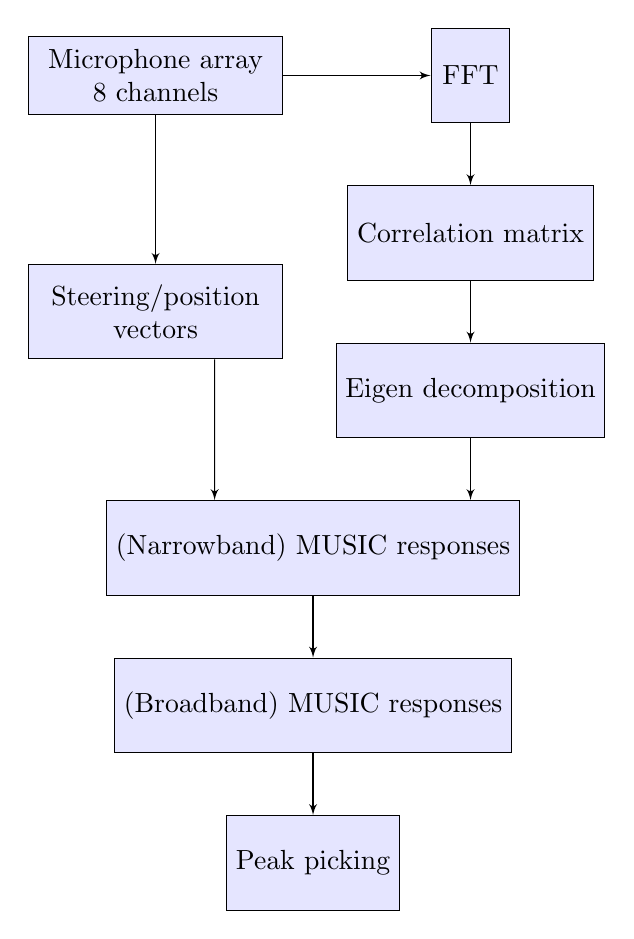
\begin{tikzpicture}[auto,node distance = 2 cm,>=latex', amp/.style = {regular polygon, regular polygon sides=3,
              draw, fill=white, text width=1em,
              inner sep=0.5mm, outer sep=0mm,
              shape border rotate=-90}
                        ]]
    % We start by placing the blocks
    \node [block, name=micro, minimum width=3cm, minimum height=1cm, text centered, text width=3cm] {Microphone array \\ 8 channels};
	\node [block, right of=micro, xshift=2cm] (fft) {FFT};    
    \node [block, below of=fft] (corr) {Correlation matrix};
    \node [block, below of=corr] (eig) {Eigen decomposition};
    \node [block,  below of=micro, yshift=-1cm, text centered, text width=3cm] (stee) {Steering/position \\ vectors};
    \node [block, below of=eig, xshift=-2cm] (mus) {(Narrowband) MUSIC responses};
    \node [block, below of=mus] (mus2) {(Broadband) MUSIC responses};
    \node [block, below of=mus2] (peak) {Peak picking};
    %\node [block,minimum height=2.2cm, minimum width=1.5cm, right of=zoh, xshift=1cm] (sat) {};
          
	% We draw an edge between the controller and system block to 
    % calculate the coordinate u. We need it to place the measurement block. 
      
    % Once the nodes are placed, connecting them is easy. 
    \draw [->] (micro) -- node[xshift=-0.5cm] {} (fft);
    \draw [->] (fft) -- node {} (corr);
    \draw [->] (corr) -- node[xshift=-1cm] {} (eig);
    \draw [->] (micro) -- node {} (stee);
    \draw [->] ([xshift=0.75cm]stee.south) -- node {} ([xshift=-1.25cm]mus.north);
    \draw [->] (eig) -- node {} ([xshift=2cm]mus.north);
    \draw [->] (mus) -- node {} (mus2);
    \draw [->] (mus2) -- node {} (peak);
     
   
\end{tikzpicture}
\caption{Block diagram of the sound source localization}
\label{fig:MUSICdiagram}
\end{figure}
\subsection{MUSIC algorithm}
\label{sec:MUSIC}
The Multiple Signal Classification algorithm can be defined as the determination of different parameters of multiple wavefronts that enter an array of antennas or sensors \cite{MUSIC}.
\\
The MUSIC algorithm provides asymptotically unbiased estimates of different parameters such as number of signals, direction of arrival (DOA), polarization, strength and cross correlation among the directional waveforms, and many others.
\newline
The $M$ array elements receive the waveforms from the sources that are linear combinations of the $D$ incidents wavefronts\footnote{explicar que es wavefront} and noise. This can be expressed as in equation \ref{equ:Xrec}.
%\begin{equation}

\begin{gather}
\label{equ:Xrec}
\begin{bmatrix}
X_1 \\ X_2 \\ \vdots \\ X_M
\end{bmatrix} = \begin{bmatrix}
\mathbf{a}(\theta_1) & \mathbf{a}(\theta_2) & \hdots & \mathbf{a}(\theta_D)
\end{bmatrix}
\begin{bmatrix}
F_1 \\ F_2 \\ \vdots \\ F_D
\end{bmatrix} + 
\begin{bmatrix}
W_1 \\ W_2 \\ \vdots \\ W_M
\end{bmatrix}  \\
 \text{or } \mathbf{X}  = \mathbf{A}\mathbf{F}+\mathbf{W} 
\end{gather}
%\end{equation}
where the vector $\mathbf{X}$ represents the $M$ received waveforms, the incident signals are represented by the vector $\mathbf{F}$ in phase and amplitude at some reference point, and the complex noise is represented by the vector $\mathbf{W}$. \\ The elements $a_{ij}$ from the matrix $\mathbf{A}$ are functions of the angle of arrival and the position of the array elements. Therefore, each element $a_{ij}$ depends on the position relative to the origin of the $ith$ array element and the response of the incident signal from the direction $jth$. The $jth$ column of matrix $\mathbf{A}$ is known as the mode vector of responses to the direction of arrival $\theta_j$ of the $jth$ signal. That is, the mode vector $\mathbf{a}_j$ is equivalently to the direction of arrival $\theta_j$.
\newline

It can be deducted from equation \ref{equ:Xrec} that the vector $\mathbf{X}$ is a linear combination of the mode vectors $\mathbf{a}(\theta_j)$ in which the elements of the matrix $\mathbf{F}$ are the coefficients of this combination. The directions of arrival of multiple incident wavefronts are calculated by determining the intersections of the $\mathbf{a}(\theta)$ continuum with the range space of $\mathbf{A}$.
\\
\newline
For determining the source localization, the correlation matrix of the input signals needs to be calculated. That is, the covariance matrix of the $\mathbf{X}$ vector is
\begin{equation}
\label{cov}
\mathbf{S}=\mathbf{X}\mathbf{X}^*=\mathbf{A}\mathbf{F}\mathbf{F}^*\mathbf{A}^*+\mathbf{W}\mathbf{W}^*.
\end{equation}
Where the * operator indicates the conjugate transpose operator. With the covariance matrix of the microphone array observations is performed a principal component analysis on this matrix to separate the disjoint signal and noise subspaces.
For these means, the eigenvalue decomposition or singular decomposition of the covariance matrix $\mathbf{S}$ is carried out. The M-th space correlation matrix obtained in \ref{cov} is decomposed in the signal and noise subspaces as per
\begin{equation}
\label{decomposition}
\mathbf{S}=\mathbf{Q}\mathbf{\Lambda}\mathbf{Q}^{-1}
\end{equation}
in which $\mathbf{Q}$ is a $M \times M$ matrix with the eigenvectors $\mathbf{q}_i$ of $\mathbf{S}$ written in the column i-th, and the matrix $\mathbf{\Lambda}$ is a diagonal matrix containing the eigenvalues. \\
The singular vectors $\mathbf{q}_i$ are orthogonal to the space spanned by the columns of $\mathbf{A}$ or in other words the vectors contained in the columns of $\mathbf{A}$ are perpendicular to each other. 
Since the eigenvectors $\mathbf{q}_i$ have correlation to the power of the incident wavefronts, the eigen vectors can be divided into $N$ noise eigenvectors and $D$ incident signal mode vectors, in which the $D$ vectors correspond to the eigenvalues with greatest value. For instance, the matrix $\mathbf{Q}$ can be written as
\begin{equation*}
\mathbf{Q}=[\mathbf{q}_1,\mathbf{q}_2,\hdots,\mathbf{q}_M]
\end{equation*}
and the split matrix gives the mode vectors \([\mathbf{q}_1,\mathbf{q}_2,\hdots,\mathbf{q}_D]\) and the noise eigenvectors \([\mathbf{q}_{1},\hdots,\mathbf{q}_{N}]\).
\newline

The next step is to solve for the incident mode vectors. In order to do that the spectrum for SSL is calculated using the noise eigenvectors as per
\begin{equation}
\label{spectrum}
P=\frac{\mid \mathbf{H}^* \mathbf{H}\mid}{\sum\limits_{i=1}^{N} \mid \mathbf{H}^*\mathbf{q}_{i} \mid}.
\end{equation} 
Where $\mathbf{H}$ is the transfer function of the sound propagation. The transfer function can be determined numerically or by measurements. The transfer function is a multichannel expression that depends on the sound $S_i$ in direction $\theta_i$ in view of the microphone array to the i-th microphone and is expressed as
\begin{equation}
\mathbf{H}=[H_1,\hdots,H_M].
\end{equation}
The transfer function is to be determined with anteriority and is also called as the steering vector.
\\
\newline
The numerator of equation \ref{spectrum} represents the multiplication between the steering vector (transfer function) and the noise-related eigenvector. This product is theoretically zero if the transfer function is a vector corresponding to the desired sound; making the quotient of the spectrum diverge infinitely. In reality, the denominator does not go exactly to zero due to the effects of noise but an abrupt peak can be observed.
\\ Equation \ref{spectrum} represents the spectrum for every frequency a broadband SSL is performed for the desired frequencies as
\begin{equation}
\hat{P}=\sum\limits_{\omega=\omega_{min}}^{\omega_{max}}W_{\Lambda}W_{\omega}P.
\end{equation}
$\omega_{min}$ and $\omega_{max}$ determine the desired frequency bands, $W_{\Lambda}$ is the eigenvalue weight and is the square root of the maximum eigenvalue. Finally, $W_{\\omega}$ is the spectrum weight factor. \\
\newline
The search of the sound is performed in the frequency bands aforementioned for $\hat{P}$ where the maxima are identified by local maximum searching or the hill-climbing method
\appendices
\section{Optionaler Titel}
Anhang eins.
\section{}
Anhang zwei.

\section{Richtlinien f�r das Verfassen wissenschaftlicher Arbeiten}
\label{sec:richtlinien}
Im Folgenden werden einige wichtige Richtlinien zusammengefasst. Die Aufz�hlung ist allerdings nicht ersch�pfend.

\begin{itemize}
 \item Klare Darstellung, was der Eigenanteil ist und was schon vorhanden war.
 \item Vorsicht vor Plagiaten: vollst�ndige Quellenangaben, auch bei Bildern. Es sollte immer klar ersichtlich sein, was der Eigenanteil ist und was aus Quellen entnommen wurde.
 \item Bilder nicht 1:1 aus Quellen kopieren.
 \item Diskussion der Ergebnisse (Simulationen, Messungen, Rechnungen): Wurde das Ergebnis so erwartet? Wenn nein, was sind m�gliche Gr�nde?
 \item Autoren: Als Autor sollte jede Person in Betracht gezogen werden, die wesentlich zur Arbeit beigetragen hat (siehe auch die Empfehlungen der DFG diesbez�glich, vgl.~\cite{wissPraxis:DFG}). Alle Personen mit kleinerem Beitrag (fachliche Hinweise, Beteiligung an Datensammlung etc.) k�nnen in der Danksagung oder einer Fu�note erw�hnt werden.
\item Formeln in den Satz einbetten und alle Variablen bei der ersten Verwendung im Text einf�hren. Beispiel:
 F�r die Temperatur ergibt sich damit
 \begin{align*}
  T(h) = K h^2,
 \end{align*}
 sie h�ngt quadratisch von der H�he $h$ ab.
\end{itemize}

\section{Hinweise zur Notation}
\label{sec:notation}
\begin{itemize}
 \item Abk�rzungen bei der ersten Verwendung erkl�ren, z.B.: ``DFG (Deutsche Forschungsgemeinschaft)''.
 \item Formelzeichen konsistent benennen, nicht zwischen den Abschnitten umbenennen. Formelzeichen kursiv schreiben, z.B. Variable $a$.
 \item Auf korrekte Dimensionen und Einheiten achten. F�r Einheiten das SI-System verwenden, z.B. das LaTeX-Paket \emph{units} oder \emph{SIunits}.
 \item Zahlen: Im Deutschen Komma als Dezimaltrennzeichen, im Englischen Punkt.
 \item Tabellen haben �berschriften, Diagramme haben Unterschriften.
 \item Diagramme: Achsenbeschriftungen hinreichend gro� (insbesondere die Zahlen).
 \item Diagrammunterschriften sollen im Wesentlichen ausreichen, um das Diagramm zu verstehen.
 \item Indizes werden \emph{kursiv} gesetzt, wenn sie die Bedeutung von Variablen haben, ansonsten \textbf{normal}. Beispiele: $V_k, \ k=1,2,\ldots$ und $V_\mathrm{input}$.
\end{itemize}




\section*{Danksagung}
Wenn ihr jemanden danken wollt, der Euch bei der Arbeit besonders
unterst�tzt hat (Korrekturlesen, fachliche Hinweise,...), dann ist hier der daf�r vorgesehene Platz.

\begin{thebibliography}{1}
\bibitem{MIT}
Ishi, C.T. et al., \emph{Evaluation of a MUSIC-based real-time sound localization of multiple sound sources in real noisy environments.},  Intelligent Robots and Systems, 2009. IROS 2009. IEEE/RSJ International Conference on. 2009. 2027-2032. �2009 Institute of Electrical and Electronics Engineers.

\bibitem{MUSIC}
R. Schmidt, \emph{Multiple emitter location and signal parameter estimation,}  in IEEE Transactions on Antennas and Propagation, vol. 34, no. 3, pp. 276-280, Mar 1986.
doi: 10.1109/TAP.1986.1143830

\bibitem{IEEEhowto:kopka}
H.~Kopka and P.~W. Daly, \emph{A Guide to {\LaTeX}}, 3rd~ed. Harlow, England: Addison-Wesley, 1999.
\bibitem{wissPraxis:DFG}
Deutsche Forschungsgemeinschaft, \emph{Vorschl�ge zur Sicherung guter wissenschaftlicher Praxis}, Denkschrift, Weinheim: Wiley-VCH, 1998.
\end{thebibliography}

\begin{biography}
[{\includegraphics[width=1in,height=1.25in,clip,keepaspectratio]{./pics/ComicKopf.eps}}] % hier ein Foto einbinden
{Autor A}
Biographie Autor A.
\end{biography}
\begin{biography}
[{\includegraphics[width=1in,height=1.25in,clip,keepaspectratio]{./pics/ComicKopf.eps}}] % hier ein Foto einbinden
{Autor B}
Biographie Autor B.
\end{biography}
\begin{biography}
[{\includegraphics[width=1in,height=1.25in,clip,keepaspectratio]{./pics/ComicKopf.eps}}] % hier ein Foto einbinden
{Autor C}
Biographie Autor C.
\end{biography}

\end{document}